\section*{Analysis}
\label{analysis}

It is possible to look at a spider plot in order to get a sense of how the speakers were rated overall, se \autoref{fig:spider_plot}. For example the BeoLab 5 overall scores the highest in the attributes: \textit{Flashy}, \textit{Decorated}, \textit{Wide}, \textit{Untypical}. This seems reasonable when presented with the speakers next to each other in \autoref{fig:speakers}. In general this paints a fitting picture over which features stands out the most and creates a unique attribute profile for each speaker when shown individually. However when shown all together as in \autoref{fig:spider_plot} a lot of points do end up close to each other and some insights may be lost due to this.

\begin{figure}[H]
\centering
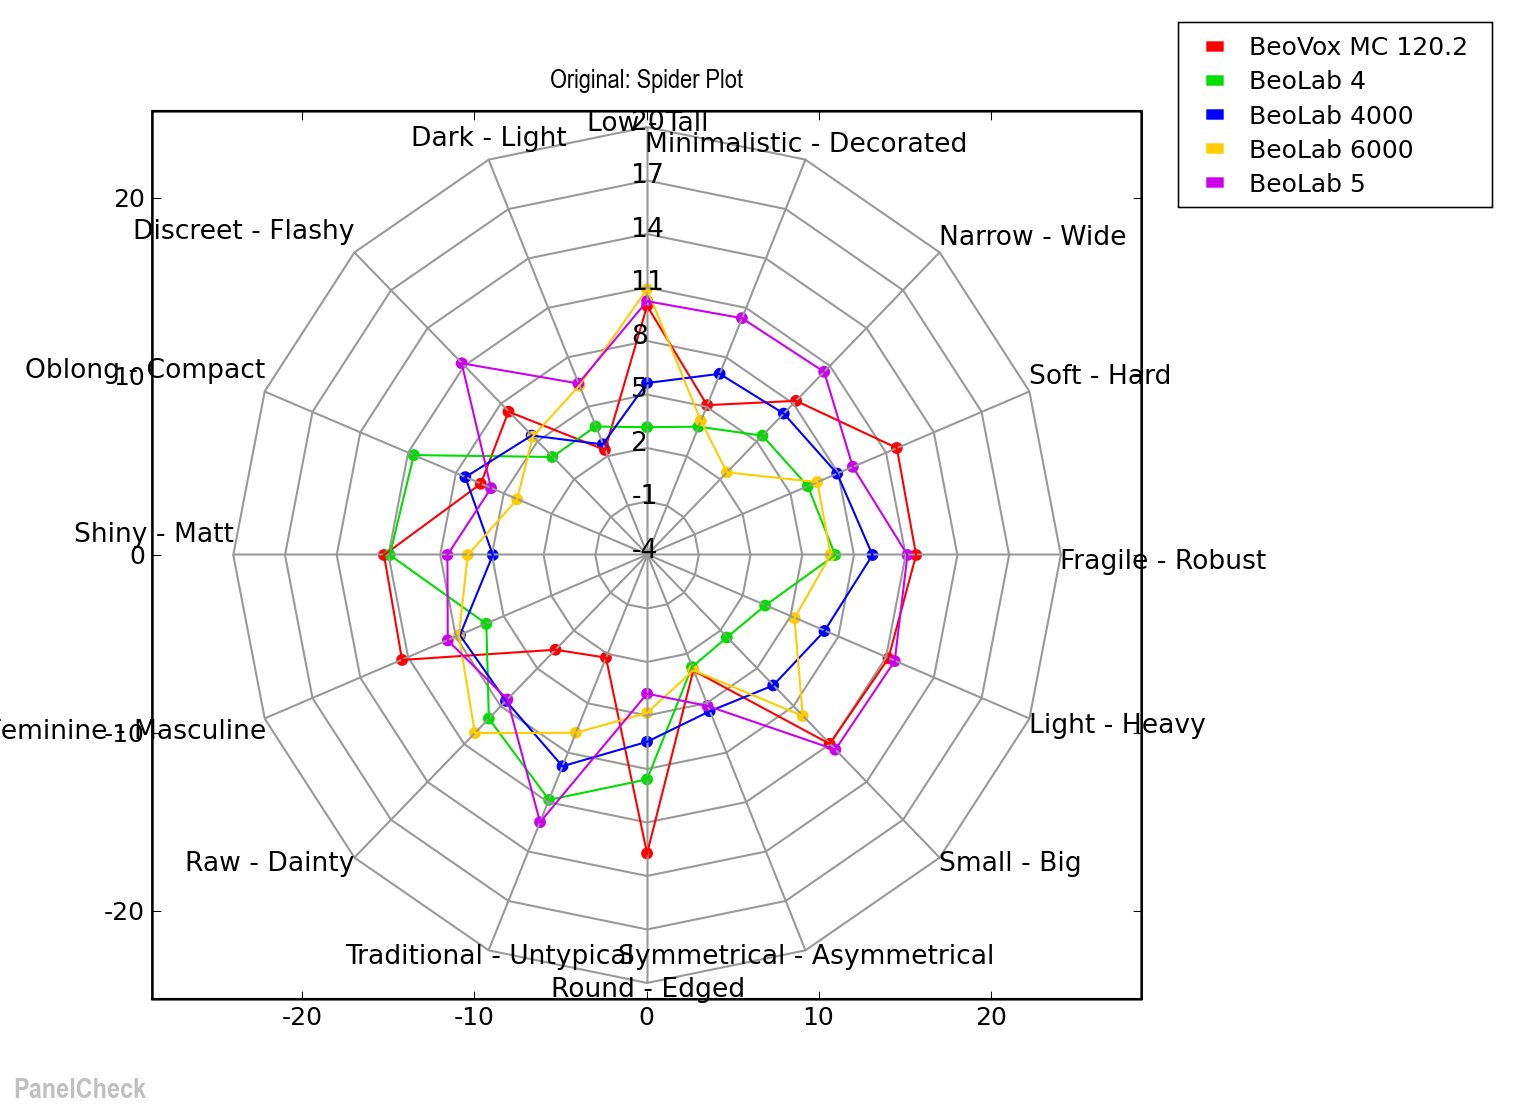
\includegraphics[width = \textwidth]{Figure/spider_plot.png}
\caption{A spider plot of the subjects' preference of the five different speakers}
\label{fig:spider_plot}
\end{figure}